\newpage\noindent
{\color{red}**}\PID
Позната је  отпорност отпорника $R = 3\unit{k\Upomega}$ и струја
успостављена на његовим прикључцима
$i = \dfrac{0,75\,I_0}{1,25 - \cos(\upomega t)}$,
где су $I_0 = 1\unit{mA}$ и $\upomega 
= 10^3\unit{\dfrac{rad}{s}}$. Израчунати средњу снагу Џулових губитака на том отпорнику, $P_R$.
\\[2mm]

\textsc{\underline{Решење}}:
Средња снага отпорника одређује се рачунањем израза
$P_R = \dfrac{1}{T}\int_{T} i^2(t) R \, \de t$. Односно,
$P_R = \dfrac{R I_0^2}{T}\int_0^T 
\left(
\dfrac{0,75}{1,25 - \cos(\upomega t)}
\right)^2
 \, \de t$. Ради једноставности, у добијеном интегралу
 се може увести смена која има смисао 
 тренутне фазе, $\upphi = \upomega t$, након чега 
се има
$P_R = \dfrac{R I_0^2}{2\uppi }\int_0^{2\uppi} 
\left(
\dfrac{0,75}{1,25 - \cos(\upphi)}
\right)^2
 \, \de \upphi$. Добијени интеграл 
\begin{equation}
I = \int_0^{2\uppi} 
\frac{0,75^2}{
\bigl(1,25 - \cos(\upphi)\bigr)^2
}
 \, \de \upphi \label{1}
\end{equation} 
 може се решити 
методама \textit{комплексне анализе.}

Косинусна функција се пре свега изражава у 
експоненцијалној форми 
$\cos(\upphi) = \dfrac{{\rm e}^{\jj \upphi}
+ {\rm e}^{-\jj \upphi}}{2}$ и замењује 
у израз \eqref{1}, након чега се сређује добијени 
израз и елиминишу негативни експоненти:
\begin{equation}
I = \int_0^{2\uppi} 
\frac{0,75^2}{
\left(1,25 - 
\dfrac{{\rm e}^{\jj \upphi}
+ {\rm e}^{-\jj \upphi}}{2}
\right)^2
}
 \, \de \upphi 
 =
\int_0^{2\uppi} 
\dfrac{2,25 \, {\rm e}^{\jj 2 \upphi} }{
(
2,5 {\rm e}^{\jj \upphi}
- {\rm e}^{\jj 2 \upphi}
- 1
)^2
}
 \, \de \upphi.
 \label{2}
\end{equation} 
\begin{slikaDesno}{fig/complex_circle.pdf}
У добијеном изразу уводи се смена $z = {\rm e}^{\jj
\upphi}$, односно $\de z = 
\jj \, {\rm e}^{\jj
 \upphi} \de \upphi$. Пошто су границе интеграције 
 за $\upphi$ од 0 до $2\uppi$ то тачка $z$ у 
 комплексној равни описује контуру $C$ јединичне 
 кружнице у позитивном математичком смеру
 (слика \ID.1).
 Трансформацијом бројиоца 
 ${\rm e^{\jj 2 \upphi}} \, \de \upphi = 
 \dfrac{z \de z}{\jj}$ и сменом 
 ${\rm e}^{\jj k \uppi} = z^k$ ($k \in \mathbb N$)
 интеграл из \eqref{2} се може записати као 
\end{slikaDesno}
 \begin{equation}
 I = 
 \dfrac{1}{\jj}
\underbrace{  
 \oint_C 
	\underbrace{	
\dfrac{2,25 z }{
(
2,5 z
- z^2
- 1
)^2
}	
	}_{f(z)}
 \,\de z
 }_{I'} \label{3}
 \end{equation}
 %\begin{wrapfigure}{l}{0.2\textwidth}
 %\vspace*{-5mm}
 % \begin{center}
 %   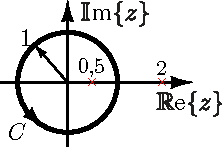
\includegraphics[width=0.2\textwidth]{fig/complex_circle.pdf}
 % \end{center}
 % \caption{Контура и полови}
 %\end{wrapfigure} 
 Контурни интеграл $I'$ се може решити
 израчунавањем резидуума полова
 подинтегралне функције, $f(z)$, који се налазе унутар 
 контуре интеграције (Кошијева теорема о 
 резидуумима): 
 \begin{equation}
 I' = \jj 2 \uppi \sum_{z_{{\rm p}k} \in C} 
 \underset{z = z_{{\rm p}k}}{\operatorname{Res}}\,
 f(z). \label{5}
 \end{equation}
 Добијена функција $f(z)$ има полове који одговарају
 коренима полинома из имениоца 
 $p(z) = 
(
2,5 z
- z^2
- 1
)^2
= (z-0,5)^2(z - 2)^2
$.
Полином има два двострука корена, 
$0,5$ и $2$, који представљају двоструке полове 
подинтегралне функције (слика \ID.1). Од ових полова, само двоструки пол
у 0,5 је унутар контуре интеграције.
Резидуум пола другог реда је у 
општем случају дат изразом 
$\underset{z = c}{\operatorname{Res}}\, f(z) 
= \lim_{z\to c} \dfrac{\de}{\de z} (z-c)^2 f(z)$. 
Израчунавањем јединог потребног резидуума се 
налази
\begin{equation}
\underset{z = 0,5}{\operatorname{Res}}\,
 f(z) = \lim_{z \to 0,5} 
 \dfrac{\de}{\de z} \left(
 \dfrac{2,25 z \cancel{(z-0,5)^2} }{
\cancel{(z-0,5)^2}(z - 2)^2
}	
 \right)
 =
 \lim_{z \to 0,5} 
 \left(
 - \frac{2,25 z + 4,5}{\left(z - 2\right)^{3}}
 \right)
 = \dfrac{5}{3}.
\end{equation}
Заменом добијеног резултата у \eqref{5} и
 \eqref{3} добија се
$I = 2\uppi \dfrac{5}{3}$ одакле се коначно заменом
у израз за снагу добија $P_R = \dfrac{RI_0^2}
{\cancel{2\uppi}} \cdot \cancel{2\uppi} \dfrac{5}{3}
= 5\unit{mW}$.

